\begin{abstract}
Rerankers in retrieval-augmented generation (RAG) systems for technical support are often adapted with weak labels derived from question--answer data. We evaluate whether one answer-aware labeling rule---ranking passages that literally contain the reference answer above other passages from the gold document---improves the answers produced by a fixed generator. We adapt Qwen3-Reranker-0.6B with LoRA on TechQA and evaluate the complete pipeline end to end with a fixed Qwen3.5-9B generator over four chunking strategies, under protocols frozen before comparative outcomes existed. On a 208-question TechQA reserve set held out from model selection (Study~1), the literal-match reranker did not significantly outperform hybrid retrieval ($\SoneDelta$ token-F1 points; 95\% CI $\SoneLow$ to $\SoneHigh$; $p=\SoneP$). In a prespecified transfer study on 273 Doc2Dial dialogue turns with three training seeds (Study~2), it was slightly worse than a reranker adapted with standard document-level labels under the same update budget ($\StwoDelta$ points; 95\% CI $\StwoLow$ to $\StwoHigh$; $p=\StwoP$) and had lower evidence NDCG@4 (\LNDCG\ vs \BNDCG). Neither study met its prespecified success criterion, and for these training runs the transfer interval excludes the targeted $+1$-point gain. Large differences in retrieval metrics translated into small differences in answer F1. The results provide no evidence that this answer-containment recipe improves generated answers in the studied setting, and they indicate that evaluations of reranker supervision should measure the final answer directly. Code and aggregate results are publicly available.
\end{abstract}
\noindent\textbf{Keywords:} retrieval-augmented generation; reranking; weak supervision; technical support; external transfer; negative results.

\section{Introduction}
Retrieval-augmented generation (RAG) systems for technical support retrieve passages from product documentation and pass them to a language model that composes the answer \citep{lewis2020}. In such systems the reranker decides which retrieved passages reach the generator, so adapting it to the target domain is a natural way to improve answer quality. Adaptation requires relevance labels, and the cheapest labels are those derived from existing question--answer data. Two derivations are common. Document-level labels mark every passage from the annotated gold document as relevant. Literal-match labels favor passages that contain the reference answer verbatim, a distant-supervision heuristic that has also been used to train dense retrievers \citep{karpukhin2020}.

Literal-match labels appear to offer a more targeted signal, because retrieving the right document does not guarantee that the selected passage contains the details a user needs. Literal containment is, however, only a lexical proxy for evidential support, and the way graded labels enter training also matters: when they are turned into contrastive training groups, gold-document passages that lack the literal answer can become negatives, and the number and weighting of groups change with the labeling rule. Whether such labels lead to better generated answers, rather than merely to different retrieval metrics, is therefore an empirical question. Related work has derived utility signals from language models or trained ranking and generation jointly \citep{shi2024,yu2024,zhang2025utility}, and has shown that query--document relevance labels can correlate only weakly with downstream RAG performance \citep{salemi2024}. Both lines of work motivate testing weak reranker supervision against the final answer rather than against retrieval metrics alone.

We test one such recipe under controlled conditions. A candidate passage receives grade~2 if it literally contains the normalized reference answer, grade~1 if it comes from a gold document but does not contain the reference, and grade~0 otherwise. Training groups pair the highest-grade passages for a question with lower-grade negatives, so gold-document passages without the literal answer can become negatives. We call this \emph{literal-match supervision} (L) and compare it with binary \emph{document-level supervision} (B), which uses gold-document membership only. Holding the retrieval pipeline, the generator and the adaptation budget fixed, we address three research questions:
\begin{enumerate}[label=\textbf{RQ\arabic*},leftmargin=3em]
\item Does a reranker adapted with literal-match labels improve generated answers over hybrid retrieval on held-out in-domain questions?
\item Under transfer to a different support domain, does literal-match supervision yield better generated answers than document-level supervision?
\item How strongly do differences in retrieval quality propagate to differences in answer F1?
\end{enumerate}

We answer these questions in two studies, each with a protocol frozen before its own comparative outcomes existed. \textbf{Study~1 (in-domain)} adapts the reranker on TechQA and compares it with hybrid retrieval on a 208-question TechQA reserve set. \textbf{Study~2 (transfer)} trains on the same TechQA development data and evaluates on 273 Doc2Dial support dialogues. It compares four methods: hybrid retrieval (H), an unadapted reranker (U), and reranker adaptation with document-level (B) or literal-match (L) labels, the latter two with three training seeds each. Both studies score the final answer from a fixed generator, and both prespecified the same success criterion: an observed gain of at least $+1$ token-F1 point with two-sided $p<0.05$.

Neither study met its criterion. Because the retrieval pipeline, generator and update budget are held fixed, these negative results are informative about the recipe itself, and the Study~2 interval excludes the targeted gain for the trained adapters. Our contributions are (i) a controlled end-to-end comparison of literal-match and document-level reranker supervision, with prespecified answer-level endpoints, transfer to a different support domain and three paired training seeds; (ii) evidence that this literal-match recipe yields lower evidence NDCG@4 than document-level supervision for every training seed, without a detectable answer-level benefit (RQ1--RQ2); (iii) diagnostics showing that large differences in retrieval metrics produced small differences in answer F1, together with a decomposition of the NDCG difference by evidence grade (RQ3); and (iv) full reporting of the unfavorable results, with post hoc analyses labeled as such and code and aggregate results released.

\section{Related work}
\subsection{Retrieval utility and supervision}
The original RAG framework combines a neural retriever with a generator for knowledge-intensive tasks \citep{lewis2020}. Later work couples retrieval more tightly to the language model: REPLUG trains the retriever with feedback from a frozen black-box language model \citep{shi2024}, and RankRAG instruction-tunes a single language model for both context ranking and answer generation \citep{yu2024}. These approaches tie retrieval supervision to generation, either through model feedback or through joint training. We instead adapt a separate reranker with fixed, deterministic weak labels and leave the generator unchanged, so that the downstream model stays fixed while the supervision rule varies.

Answer containment is a classic distant-supervision signal. Dense Passage Retrieval uses passages that contain the answer as positives when gold passages are not annotated \citep{karpukhin2020}, and FILCO selects useful context for RAG with string inclusion, lexical overlap and conditional cross-mutual information before training a context filter \citep{wang2023filco}. eRAG shows that query--document relevance labels correlate only weakly with downstream RAG performance and instead labels each retrieved document by the quality of the answer generated from it \citep{salemi2024}, which implies that relevance labels and downstream utility can diverge. Our study applies the containment heuristic to reranker adaptation and tests directly whether it improves the generated answer.

The closest supervision comparison is the utility-focused annotation study of \citet{zhang2025utility}, which trains on MS MARCO-derived data with LLM-generated utility annotations and a loss that accommodates multiple positives through summed marginal likelihood. Our labels are deterministic string-match proxies, and our training builds a separate positive-first group for each highest-grade candidate, so each positive is scored only against lower-grade negatives in its own group rather than sharing probability mass with the other positives in a single objective. Our non-significant answer-level result therefore concerns this particular literal-match recipe and the training groups it induces, not LLM utility annotation or semantic support supervision in general.

We build on existing components, the Qwen3 reranker family \citep{zhang2025qwen} and low-rank adaptation (LoRA) \citep{hu2021}, and make no state-of-the-art claim. \citet{wang2024} examine configuration choices across a broader RAG pipeline, and \citet{cuconasu2024} show that the composition of the retrieved context can itself affect generation quality. Our study is narrower and complementary: a controlled comparison of reranker supervision with an answer-level primary outcome.

\subsection{Datasets and evaluation}
TechQA was introduced for domain-specific technical question answering \citep{castelli2020}; we use a pinned NVIDIA RAG-oriented distribution with 608 eligible questions, whose split sizes differ from those of the original paper. Doc2Dial provides document-grounded support dialogues \citep{feng2020}. We select one user-to-agent transition per document, use the next agent utterance as the generation reference, and keep the annotated grounding spans as a separate retrieval target.

RAGAs and ARES assess retrieval and context properties separately from generated-answer quality using automated judges \citep{es2024,saad2024}. We likewise keep these constructs apart but use no model-judge scores: literal containment, answer token F1 and grounding-span overlap are reported as distinct measurements. Following \citet{dror2018}, our statistical tests treat the question or document, not the repeated chunker and seed records, as the unit of analysis.

\section{Methods}\label{sec:pipeline}
Figure~\ref{fig:design} summarizes the design. The following subsections describe the shared retrieval and generation pipeline, the two supervision rules and the training groups they induce, training and model selection, and the supporting use of AI tools.
\begin{figure}[htbp]\centering
\begin{tikzpicture}[
  box/.style={draw=black!60, rounded corners=2pt, align=center, font=\small, inner sep=5pt,
              execute at begin node={\hyphenpenalty=10000}},
  study/.style={box, fill=black!4},
  arr/.style={-{Stealth[length=2.2mm]}, black!70, thick}]
\node[box, text width=3.5cm] (data) {\textbf{TechQA development}\\400 questions\\(200 train, 200 validation)};
\node[box, text width=8.2cm, right=0.8cm of data] (adapt) {\textbf{LoRA adaptation of Qwen3-Reranker-0.6B}\\
  B: document-level labels; L: literal-match labels\\
  Study~1: L, one seed; Study~2: B and L, three seeds each};
\node[study, text width=5.6cm, below=0.9cm of data.south west, anchor=north west] (s1)
  {\textbf{Study 1 (in-domain)}\\TechQA reserve, 208 questions\\Compare L with H};
\node[study, text width=5.6cm, right=0.8cm of s1] (s2)
  {\textbf{Study 2 (transfer)}\\Doc2Dial, 273 dialogue turns\\Compare H, U, B and L (primary: L vs B)};
\node[box, text width=12.6cm, below=0.8cm of s1.south west, anchor=north west] (pipe)
  {Each method: hybrid retrieval (BM25 + dense, 20 candidates, four chunkers) $\rightarrow$ rerank $\rightarrow$ top four passages\\
   $\rightarrow$ fixed Qwen3.5-9B generator $\rightarrow$ answer token F1 against the reference};
\draw[arr] (data) -- (adapt);
\draw[arr] (adapt.south) -- ++(0,-0.35) -| (s1.north);
\draw[arr] (adapt.south) -- ++(0,-0.35) -| (s2.north);
\draw[arr] (s1.south) -- (s1.south |- pipe.north);
\draw[arr] (s2.south) -- (s2.south |- pipe.north);
\end{tikzpicture}

\caption{Study design. Rerankers are adapted on TechQA development data and evaluated end to end with the same retrieval pipeline and a fixed generator. Study~1 used an earlier training pipeline and one seed; Study~2 trains B and L under a shared configuration with three seeds each.}\label{fig:design}
\end{figure}
\subsection{Retrieval and generation pipeline}
For each question (Study~1) or dialogue-history query (Study~2), sparse BM25 and dense retrieval are combined by weighted reciprocal-rank fusion (weights 0.4 sparse and 0.6 dense; fusion constant 60). Dense retrieval uses BAAI/bge-small-en-v1.5 with its query prefix. Each channel retrieves 20 passages; fusion ranks their union, with a missing channel contributing zero, and retains a common pool of 20 per query and chunker. Exact fusion ties preserve dense-channel insertion order, followed by sparse-only candidates. Four fixed chunkers are evaluated: fixed 128 tokens with 19-token overlap, fixed 254 tokens with 38-token overlap, recursive 254 tokens with 38-token overlap, and sentence-based 254 tokens without overlap, with token limits from the all-MiniLM-L6-v2 tokenizer.

At inference, the methods differ only in how they order this common pool. H returns the hybrid ranking; U reranks the pool with the unadapted Qwen3-Reranker-0.6B; B and L rerank it with LoRA adapters on the same model. Each method passes its top four passages to a fixed Qwen3.5-9B generator (greedy decoding, thinking disabled, bfloat16, at most 1,536 input and 512 new tokens, batch size four). The reranker instruction asks for passages with sufficient answer evidence; this wording does not make the training labels semantic sufficiency judgments. Exact model revisions are listed in \supp{S2}{supp:impl}.

Long inputs are handled differently at each stage. Dense queries are truncated on the right at 512 tokens, including special tokens, so a long history can lose its latest turns. Reranker inputs are also right-truncated to 512 tokens, which cuts the end of an overlength passage first, whereas training pruned such pairs. Generator packing instead preserves the full history and removes the context suffix. The numbers of truncated retrieval and reranker inputs were not recorded (\supp{S2}{supp:impl}).

\subsection{Supervision labels and training groups}
The two supervision rules differ in how they grade candidate passages and, as a consequence, in the training groups they induce. Let $D_q$ be the annotated gold-document set for TechQA training question $q$, $d(c)$ the document containing candidate passage $c$, and $A(q,c)$ an indicator that the normalized reference answer occurs as a contiguous token sequence in $c$. Document-level supervision is
\begin{equation}
 b(q,c)=\mathbf{1}\{d(c)\in D_q\}.
\end{equation}
Normalization lowercases, deletes ASCII punctuation, removes the English articles ``a'', ``an'' and ``the'', and collapses whitespace; it does not perform Unicode normalization, stemming or partial-reference matching. A chunk containing only part of every reference does not satisfy $A$. Literal-match supervision assigns
\begin{equation}
 \ell(q,c)=\begin{cases}2,&A(q,c)=1,\\1,&A(q,c)=0\text{ and }d(c)\in D_q,\\0,&\text{otherwise}.\end{cases}
\end{equation}
The literal test takes precedence, so grade~2 does not also require gold-document membership. In the study protocol and the released files, L is named ``evidence-specific'' (condition E), and the Study~1 system ``evidence-aware''; we use L throughout.

Training groups are built from the pooled candidates of all four chunkers, which are deduplicated on exact normalized text. Representatives are chosen by fused rank, then chunker priority (fixed-128, fixed-254, recursive-254, sentence-254), then identifier; group construction orders candidates by fused rank, then identifier. Nonidentical overlapping passages remain separate. The highest grade present defines the positives, and lower-grade candidates supply up to seven negatives in fused-rank order. Each positive forms its own group with these negatives; questions without both a positive and a lower-grade negative form no group. Under L, gold-document passages are therefore eligible negatives whenever a literal-match passage exists; when none exists, L falls back to grade-1 positives. In Study~2, deduplication ignores labels, pairs exceeding 512 tokens under the actual training template are pruned, and a group needs an in-limit positive and at least one surviving negative. Table~\ref{tab:toy} illustrates the difference on a small constructed pool.

The resulting inventories contain 2,103 B and 943 L training groups and 4,019 B and 1,799 L groups for the final refits. A retrospective inventory audit found usable groups for 189/187 of 200 training questions and 379/376 of 400 refit questions (B/L). Only 22.5\% of L training groups and 23.9\% of L refit groups have grade-2 positives; the rest use grade-1 fallback. In those grade-2 groups, grade-1 passages occupy 51.8\% and 52.2\% of negative positions, respectively. Out-of-document literal matches produce three usable positive groups across two questions in each split (full counts in \supp{S2}{supp:impl}).
\begin{table}[htbp]\centering\small
\caption{Constructed example (not from the data) of how B and L label one candidate pool and which training groups result. The reference answer is ``restart the monitoring agent''. A group is written as (positive; negatives).}\label{tab:toy}
\begin{tabular}{lp{0.55\linewidth}cc}\toprule
Passage & Content & B & L\\\midrule
$c_1$ & Gold document; contains ``restart the monitoring agent'' & 1 & 2\\
$c_2$ & Gold document; describes the agent's log settings & 1 & 1\\
$c_3$ & Gold document; lists supported versions & 1 & 1\\
$c_4$ & Other document; contains ``restart the monitoring agent'' & 0 & 2\\
$c_5$ & Other document; unrelated product & 0 & 0\\\midrule
\multicolumn{4}{l}{B groups: $(c_1;\,c_4,c_5)$, $(c_2;\,c_4,c_5)$, $(c_3;\,c_4,c_5)$}\\
\multicolumn{4}{l}{L groups: $(c_1;\,c_2,c_3,c_5)$, $(c_4;\,c_2,c_3,c_5)$}\\\bottomrule
\end{tabular}\end{table}

For each group $g$, positions $j=0,\ldots,m_g$ index one positive ($j=0$) and $1\le m_g\le7$ surviving lower-grade negatives. With score $s_{gj}$ (the final-token yes-minus-no logit), Study~2 minimizes
\begin{equation}
 \mathcal L=-\frac{1}{|\mathcal G|}\sum_{g\in\mathcal G}\log\frac{\exp(s_{g0})}{\sum_{j=0}^{m_g}\exp(s_{gj})}.
\end{equation}
Groups are shuffled each epoch and drawn until a fixed update budget is reached, so questions with more positives contribute more groups. Equal budgets therefore do not imply equal exposure: each final refit draws 1,724 groups (431 updates of four groups), about 0.43 passes over B's 4,019 groups but 0.96 passes over L's 1,799. B and L thus differ in which questions form groups and how often each group is seen, not only in their label values. We compare these complete supervision pipelines and do not isolate the effect of the labels alone.

\subsection{Training and model selection}\label{sec:training}
Study~2 uses rank-16 LoRA (alpha 32, dropout 0.05, all linear layers), AdamW with weight decay 0.01, warmup ratio 0.1, gradient clipping at 1 and four groups per update. A development grid crosses two learning rates ($5\times10^{-5}$, $10^{-4}$), three update budgets (227, 454, 681) and B/L, giving 12 jobs with seed 20260904. The selected configuration maximizes the average of the B and L validation NDCG@4 over 200 validation questions and four chunkers, with ties broken toward fewer updates and then the lower learning rate. Each method's validation NDCG uses its own training grades (binary for B, three-level for L), so the two values are not directly comparable; Section~\ref{sec:discussion} compares them on common grades. The selected configuration is $10^{-4}$ with 227 updates (validation NDCG@4 0.838 for B and 0.810 for L, each on its own grades). Independent own-grade selection would retain this configuration for B but choose $5\times10^{-5}$ with 227 updates for L (0.817 on L grades); no transfer outcomes exist for that alternative refit. The shared-budget rule is therefore part of the tested pipeline, not evidence of individually optimal training. Because every grid budget gives L about 2.2 times as many passes over its smaller group inventory as B, shared selection also couples the learning rate with exposure (\supp{S2.4}{sec:validationgrid}).

A frozen lookup sets the final-refit updates ($227\mapsto431$, $454\mapsto862$, $681\mapsto1{,}293$); its original derivation was not retained. Retrospectively, the values equal $k\lceil 907/4\rceil$ and $k\lfloor 1{,}725/4\rfloor$ for $k=1,2,3$, that is, one to three passes of four-group updates over Study~1's surviving training and refit groups. This arithmetic correspondence is a reconstruction, not a recovered record, and it rounds up for training but down for refits (\supp{S2}{supp:impl}). Final refits on all 400 development questions used seeds 20260904, 20260905 and 20260906.

Study~1 used an earlier training pipeline: grade-aware deduplication, deletion of whole groups with overlength inputs, and a different training framework. Its six development adapters cross two learning rates and one to three epochs; $10^{-4}$ and three epochs were selected (validation NDCG@4 0.809). Its comparator is hybrid retrieval, chosen on development data, rather than B. No configuration in either study was chosen using reserve or Doc2Dial answer outcomes.

\subsection{Use of AI tools in the analysis}
The study design, experimental pipeline, model training, evaluation runs and primary analyses were carried out by the authors. AI coding agents (OpenAI Codex, GPT-5.x and GPT-6.x series models, during the earlier revision; Claude Code with Claude Opus 5.5, Anthropic, during the final revision) were used in a supporting role to script the retrospective checks and post hoc diagnostics that recompute values from saved records, such as the sensitivity calculations, split-rule recomputation, exposure breakdown and grade-composition diagnostics (\supp{S1}{supp:register}, \supp{S2}{supp:impl}, \supp{S4}{supp:study1}, \supp{S5}{sec:s5}). The authors reviewed this code and its outputs.

\section{Experimental design}
\subsection{Study 1: in-domain TechQA}
The pinned TechQA distribution yields 608 eligible questions and 496 documents, split by a salted-hash rule into 200 training, 200 validation and 208 reserve questions (\supp{S2}{supp:impl}). The reserve was excluded from Study~1 training, validation, comparator choice and hyperparameter selection. It was not untouched, however: earlier project work had produced artifacts for 152 of the 208 reserve questions (Section~\ref{sec:limitations}).

The primary outcome is the per-question difference in answer token F1 between L and H, averaged over the four chunkers. Only training seed 20260904 has complete answer generation (832 outputs per condition); seeds 20260905 and 20260906 have retrieval results only. The 95\% interval is a percentile interval from 20,000 question-bootstrap draws, and the two-sided $p$-value comes from 100,000 paired sign flips. A post hoc exposure breakdown gives $+0.16$ F1 points for the 56 questions without a discovered prior artifact and $+0.88$ for the 152 with prior artifacts; because these subsets are not randomized, the difference does not establish a contamination effect (\supp{S4}{supp:study1}). Reserve NDCG values use a corrected normalization (\supp{S4}{supp:study1}); the correction does not change rankings, generated answers or F1.

\subsection{Study 2: transfer to Doc2Dial}
Because a demonstrably unexposed TechQA evaluation set could not be established, Study~2 evaluates transfer to IBM Doc2Dial v1.0.1. A deterministic salted-hash rule selects one eligible user turn and the following agent response from each eligible validation document, giving 273 documents (DMV 51, SSA 77, student aid 50, VA 95; rule and salt in \supp{S2}{supp:impl}). An eligible transition has a user turn immediately followed by an agent turn with a nonblank response and nonempty grounding references; every document represented in the validation dialogues has one. Retrieval searches all 488 documents across the four domains; documents outside the validation population are searchable but not evaluated. The query is the dialogue history up to and including the selected user turn; the target response, later turns, gold-document identifiers and grounding spans are unavailable at inference time.

The primary reference is the selected agent utterance, and token F1 against it (response F1) is the primary outcome; F1 against the grounding span (span F1) is secondary. For retrieval evaluation, a passage receives grade~2 if it contains any nonempty normalized grounding span as a character substring, without requiring gold-document membership; unlike TechQA's token-subsequence test, this can match within a word. Otherwise it receives grade~1 if it belongs to the gold document, and~0 otherwise. We refer to NDCG@4 under these grades as evidence NDCG@4. Before the protocol was frozen, only dataset metadata and the selection index had been examined; no comparative H/U/B/L outcomes existed.

For document $d$, the primary statistic averages the $L-B$ F1 difference over four chunkers $c\in\{1,\ldots,4\}$ and three paired training seeds $s\in\{1,\ldots,3\}$:
\begin{equation}
 \Delta_d=\frac{1}{12}\sum_{c=1}^4\sum_{s=1}^3\left(\Fone_{L,d,c,s}-\Fone_{B,d,c,s}\right),\qquad
 \widehat\Delta=\frac{1}{273}\sum_{d=1}^{273}\Delta_d.
\end{equation}
Within each domain, documents whose titles match after normalization (lowercasing and removing trailing numbered suffixes) form a dependency family; there are 235 families. The 95\% interval uses 20,000 bootstrap draws that resample whole families within domains; each draw divides the resampled document sum by the realized document count $N^*$, which varies as unequal-size families are repeated (\supp{S1}{supp:register}). The two-sided $p$-value uses 100,000 sign flips with one sign per family.

\subsection{Secondary and exploratory analyses}
Prespecified secondary summaries for Study~2 are domain effects, an equal-domain mean, per-seed effects with their spread and leave-one-seed-out values, retrieval metrics and operational measurements; response exact match and span F1 are also reported. All are descriptive. An earlier planning proposal described a five-comparison Holm family, but both frozen protocols list descriptive secondary summaries instead, and we follow the frozen protocols (\supp{S1}{supp:register}). All pairwise method contrasts, per-chunker breakdowns, top-four overlap and evidence-flow associations come from a post-study exploratory specification dated 8 September 2026 and carry no $p$-values.

For returned grades $g_1,\ldots,g_4$ and the four largest pool grades $g^*_1,\ldots,g^*_4$,
\begin{equation}
\mathrm{DCG}@4=\sum_{i=1}^4\frac{2^{g_i}-1}{\log_2(i+1)},\qquad
\mathrm{NDCG}@4=\begin{cases}\mathrm{DCG}@4/\mathrm{IDCG}@4,&\mathrm{IDCG}@4>0,\\0,&\mathrm{otherwise},\end{cases}
\end{equation}
where IDCG substitutes $g_i^*$ in the same sum. Zero-IDCG cells remain in the mean denominator. The ideal ranking is restricted to the common 20-candidate pool. A retrospective normal-reference sensitivity analysis gives approximate 80\%-power detectable gains of 1.47 F1 points for Study~1 and 1.18 for Study~2 under the compound success rule. These conditional, observed-variance approximations are not exact sign-flip-test power or prospective design claims; \supp{S1}{supp:register} separates them from the original planning assumptions.

\section{Results}
\subsection{Primary outcomes}
Neither study met its success criterion (Figure~\ref{fig:primary}); the two studies are not pooled. In Study~1, mean answer F1 was \SoneH\ for H and \SoneL\ for L, a difference of $\SoneDelta$ points computed from unrounded means (95\% CI $\SoneLow$ to $\SoneHigh$; $p=\SoneP$). The per-question differences were small and mixed: L was better on 115 questions, worse on 86 and tied on 7 (Cohen's $d_z=0.09$). Neither the $+1$-point threshold nor the significance condition was met, and exact match was rare (1 of 832 H outputs and 4 of 832 L outputs). Because the interval extends from a small loss to gains above the target, Study~1 neither demonstrates nor excludes a one-point improvement.

In Study~2, the $L-B$ difference in response F1 was $\StwoDelta$ points (95\% CI $\StwoLow$ to $\StwoHigh$; $p=\StwoP$). The success criterion was not met, and the interval, which conditions on the three trained seed pairs, excludes the targeted $+1$-point gain. Study~2 therefore gives the more decisive negative result: conditional on these trained adapters, a gain of the targeted size lies outside the 95\% interval, although the interval does not establish that the two supervision rules are equivalent.
\begin{figure}[htbp]\centering
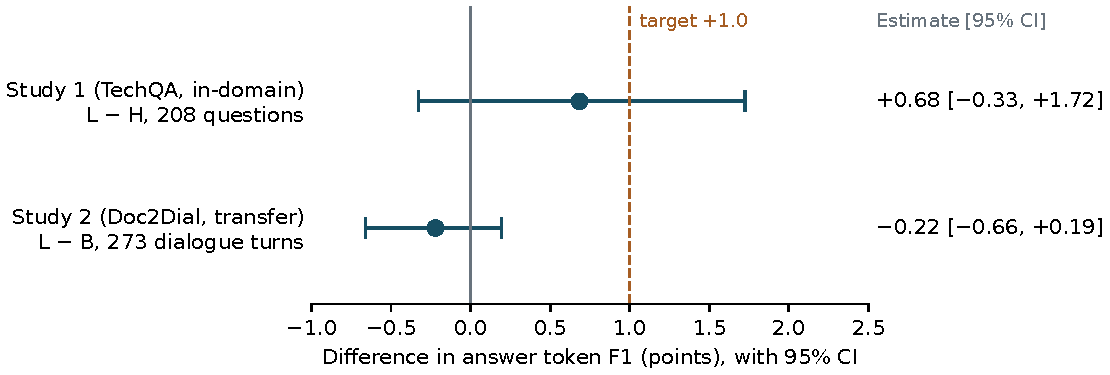
\includegraphics[width=\linewidth]{figures/primary_forest.pdf}
\caption{Primary estimates with 95\% intervals, in answer token-F1 points. Study~1 averages four chunkers per question with one generation seed (question bootstrap). Study~2 averages four chunkers and three paired training seeds per document (family bootstrap over 235 families). The dashed line marks the targeted $+1$-point gain.}\label{fig:primary}
\end{figure}

\subsection{Method means and variation in Study 2}
Table~\ref{tab:methods} reports all four Study~2 methods. All three reranking methods exceed H in response F1, but adaptation adds little beyond the unadapted reranker: B exceeds U by only 0.02 response-F1 points, and L is 0.20 points below U. Evidence NDCG@4 separates L from the other methods more clearly: L (\LNDCG) is below B (\BNDCG), U (\UNDCG) and H (\HNDCG). These descriptive differences show no answer-quality benefit of either adaptation recipe over the unadapted reranker, although they do not establish equivalence.
\begin{table}[htbp]\centering\small
\caption{Study 2 method means. F1 and exact match (EM) in points; NDCG@4 on the 0--1 scale. H/U: 1,092 records each; B/L: 3,276 each (three training seeds).}\label{tab:methods}
\begin{tabular}{lrrrr}\toprule
Method & Response F1 & Span F1 & Response EM & NDCG@4\\\midrule
H & 23.57 & 22.65 & 0.00 & 0.650\\
U & 24.03 & 23.30 & 0.18 & 0.686\\
B & 24.05 & 23.24 & 0.06 & 0.689\\
L & 23.83 & 23.12 & 0.06 & 0.612\\
\bottomrule\end{tabular}\end{table}


The direction of the primary contrast is consistent across domains but not across seeds. All four domain effects are negative (Table~\ref{tab:domains}), with an equal-domain mean of $-0.26$ points. The per-seed effects differ in sign (Table~\ref{tab:seeds}; standard deviation 0.49 points, range $-0.53$ to $+0.35$), yet every leave-one-seed-out mean is negative. The positive effect at seed 20260904, which was also the grid-selection seed, reflects B's lowest seed mean (23.61 points, versus 24.42 and 24.11) rather than an unusually high L mean (23.58--23.96 across seeds; \supp{S3}{supp:study2}). By contrast, the $L-B$ NDCG contrast is negative for all three seeds, so the sign change in answer F1 is not accompanied by a sign change in retrieval NDCG. Chunker effects are $-0.26$ (fixed-128), $-0.04$ (fixed-254), $-0.99$ (recursive-254) and $+0.41$ (sentence-254) points. Full method means by domain, chunker and seed are in \supp{S3}{supp:study2}.
\begin{table}[htbp]\centering\small
\caption{Study 2 $L-B$ response-F1 difference by domain (points). The equal-domain mean weights domains equally; the primary estimand weights documents equally.}\label{tab:domains}
\begin{tabular}{lrr}\toprule
Domain & Documents & $L-B$ F1\\\midrule
DMV & 51 & $-$0.63\\
SSA & 77 & $-$0.11\\
Student aid & 50 & $-$0.18\\
VA & 95 & $-$0.11\\
Equal-domain mean & 273 & $-$0.26\\
\bottomrule\end{tabular}\end{table}

\begin{table}[htbp]\centering\small
\caption{Study 2 $L-B$ response-F1 differences (points), leave-one-seed-out means, and retrieval NDCG@4 differences (0--1 scale). Seed 20260904 was also used for development-grid selection.}\label{tab:seeds}
\begin{tabular}{lrrr}\toprule
Seed & $L-B$ F1 & Without this seed & $L-B$ NDCG@4\\\midrule
20260904 & $+0.35$ & $-0.51$ & $-0.0827$\\
20260905 & $-0.48$ & $-0.09$ & $-0.0551$\\
20260906 & $-0.53$ & $-0.07$ & $-0.0937$\\
\bottomrule\end{tabular}\end{table}


\subsection{From retrieval to answers}\label{sec:propagation}
Differences in retrieval metrics translate into much smaller differences in answer F1. Reranking itself ($U-H$) raises evidence NDCG@4 by 0.036 but answer F1 by only 0.46 points, and the 0.077 NDCG@4 deficit of L relative to B corresponds to an F1 difference of only $-0.22$ points (\supp{S3}{supp:study2}). Three descriptive observations help characterize these differences.

First, B and L select from pools that usually contain literal evidence, and they choose broadly similar passages. Of 1,092 query--chunker pools, 874 contain at least one passage with a literal annotated grounding span, and 57 contain no graded passage at all. B and L share on average 67\% of their top four; the sets are identical in 20\% of paired cells and the order in 5\%. The fraction of packed contexts with a literal annotated span is 0.658 for H, 0.701 for U, 0.704 for B and 0.670 for L, and no selected span is lost when passages are packed into the prompt.

Second, a post hoc analysis of the saved rankings shows that L selects fewer gold-document passages without a literal span (grade~1) and more passages without any graded evidence (grade~0). Grade-1 passages occupy 27.2\%, 27.5\%, 27.8\% and 24.2\% of the top-four slots for H, U, B and L; grade-0 shares are 48.1\%, 46.1\%, 46.0\% and 50.8\%. L selects slightly more grade-2 passages than H (mean 0.999 vs 0.986 per top four), yet its NDCG is lower: grade-1 normalized-DCG losses account arithmetically for 82.0\% of the $-0.0379$ $L-H$ difference (four-decimal values in this paragraph are computed from unrounded means; \supp{S5}{sec:s5}). Against B, grade-1 and grade-2 contributions are $-0.0348$ and $-0.0423$, jointly accounting for the $-0.0772$ difference (0.689 vs 0.612 after rounding). In the 161 grade-1-only pools, the $L-B$ NDCG difference is $-0.1427$ while the F1 difference is $+0.73$ points; in the 874 grade-2-available pools the differences are $-0.0701$ and $-0.39$ points. The 57 zero-grade pools contribute zero NDCG but remain in F1 summaries. These are descriptive decompositions, not evidence that negative inversion caused the deficit (full strata and seed-weighting rules in \supp{S5}{sec:s5}).

Third, at the document level, answer-F1 differences track generated length more closely than retrieval quality. For each of the 273 documents, we first average each $L-B$ metric difference uniformly over its 12 chunker-by-seed cells. Across those paired document means, the NDCG@4 difference correlates only weakly with the response-F1 difference (Pearson $r=0.22$; Spearman $\rho=0.18$), whereas the difference in generated length is more strongly and negatively associated with it ($r=-0.35$; $\rho=-0.47$). With the F1 metric's normalized whitespace tokenizer, reference utterances average 16.31 tokens (median 14), while generated answers average 63.80, 65.60, 64.43 and 64.57 tokens for H, U, B and L. In these metric tokens, macro precision is 0.179--0.182 and recall 0.516--0.532 (\supp{S5}{sec:s5}). For token F1 with positive reference overlap, adding nonoverlapping tokens lowers precision and F1 without lowering recall; the length association therefore need not indicate worse semantic support. These associations are descriptive, and all of them are listed in \supp{S5}{sec:s5}.

The generation records are consistent with the prompt budget. Mean generated lengths are 88.5, 91.3, 89.8 and 90.0 Qwen tokenizer tokens for H, U, B and L (a different unit from the metric tokens above); two outputs (one each for B and L) reach the 512-token cap. The prompt-budget audit covered all 8,736 packing cases: five contexts were truncated and none exceeded 1,536 input tokens. The audit reconstructed input lengths rather than relying on a legacy saved field, which is invalid for 5,958 records (H/U: 745 each; B/L: 2,234 each; \supp{S5}{sec:s5}).

\section{Compute cost}
Study~2 used 46,280 allocated A100-seconds (12.86 A100-hours, within the planned 20-hour budget), including loading, I/O, failures and retries. This total covers 12 grid jobs, 12 validation runs, six final refits, 1,092 retrieval cells, 152,880 reranker scores and 8,736 generated answers; development smoke tests and earlier project compute are not included. Batched unadapted reranking scored 164.2 steady-state pairs/s, excluding the first 32 of 21,840 scored pairs (1.05\,s base loading). Each adapted run also scored 21,840 pairs (21,808 in its steady-state denominator): B and L achieved 91.6--91.7 pairs/s, with base loading of 1.02--1.07\,s and adapter loading of 0.44--0.47\,s per instance (131,040 adapted pairs in total; full per-seed measurements in \supp{S6}{supp:cost}). The final generation session produced 29,912 tokens for 300 records in 614.5\,s (48.7 tokens/s), with 231.4\,s of model loading reported separately. The reranker timers cover synchronized forward passes after tokenization and device transfer. These are component measurements, not per-request latencies or a matched serving comparison. Operational fixes made during the run are documented in \supp{S6}{supp:cost}.

\section{Discussion}\label{sec:discussion}
\paragraph{What the experiments establish.} The two studies answer RQ1 and RQ2 consistently: literal-match supervision did not produce a demonstrable improvement in generated answers. Study~1 yields a small positive estimate against hybrid retrieval ($\SoneDelta$ points), but its interval includes zero, its criterion fails and its reserve was partly exposed in earlier work. Study~2 asks the sharper question, literal-match versus document-level labels under transfer, and gives a slightly negative estimate ($\StwoDelta$ points) whose interval excludes the targeted gain. Retrieval quality did not improve either: L had the lowest evidence NDCG@4 of the four methods, and its deficit relative to B appeared for every training seed. Because the retrieval pipeline, generator and update budget were held fixed and the protocols were frozen before comparative outcomes existed, these negative results are informative about this recipe; they do not, however, establish that the two supervision rules are equivalent.

\paragraph{Possible explanations for the retrieval deficit.} L's retrieval deficit already appears in-domain, before transfer. In a post hoc re-scoring of the saved TechQA validation rankings on L's own three-level grades, L was below B at the selected configuration (NDCG@4 0.810 vs 0.824; difference $-0.013$, 95\% question-bootstrap CI $-0.026$ to $-0.001$; L lower on 75 and higher on 42 of 200 questions) and in five of the six grid configurations; the best L run (0.817) was also below the best B run (0.824) (\supp{S2.4}{sec:validationgrid}). This analysis uses one training seed and was not in the protocol, so it is suggestive rather than confirmatory. Two features of the recipe could explain such a deficit. First, under L, grade-1 gold-document passages that lack the literal answer are eligible negatives, which may teach the reranker to demote useful passages. Only 22.5\% of L's training groups (23.9\% of refit groups) have such grade-2 positives; the rest fall back to grade-1 positives against grade-0 negatives, as in B, so most L groups carry no literal-match signal. The lower share of grade-1 passages in L's top four under transfer (24.2\% versus 27.8\% for B; Section~\ref{sec:propagation}) is consistent with this mechanism but, as a descriptive decomposition, does not establish it. Second, the fixed budget covers a larger fraction of L's smaller group set (0.96 vs 0.43 passes); at the selected budget neither method completes its first pass. The group construction also changes question weights. These exposure differences prevent attributing the contrast to label granularity alone, and the shared selection rule couples them with the learning rate: L's own-grade optimum used the lower learning rate, for which no transfer outcome exists (Section~\ref{sec:training}). Transfer also changes the literal proxy from technical-answer strings to grounding-span strings, while answer F1 targets conversational utterances; this construct shift may add to the in-domain deficit. The study does not isolate these explanations. A future development-only comparison could hold candidate pools, question weights and exposure fixed while comparing multi-positive marginal likelihood \citep{zhang2025utility} or a graded ranking objective such as LambdaLoss \citep{wang2018lambda}. Such ablations would require new experiments and an evaluation population independent of the observed Doc2Dial outcomes.

\paragraph{Weak propagation from retrieval to answers.} The answer metric responds weakly to retrieval (RQ3). Reranking as a whole moved F1 by less than half a point, so the $+1$-point target was demanding: it was about twice the gain from reranking itself. Under the retrospective normal-reference approximation, even a true one-point gain would have met the compound success rule with a probability of only approximately 47.7\% in Study~1 and 50.0\% in Study~2 (\supp{S1}{supp:register}). The negative association between length and F1 differences suggests that token F1 here is also sensitive to verbosity, and the weak document-level correlation between NDCG and F1 differences ($r=0.22$) is consistent with the finding that relevance-based retrieval evaluation correlates only weakly with downstream RAG performance \citep{salemi2024}. Future studies of reranker supervision would benefit from calibrating the answer metric first, for example with oracle-context and no-retrieval conditions, before choosing a target effect. Native multi-document dialogue tasks such as MultiDoc2Dial \citep{feng2021multi} would test a different conversational setting but require a fresh, exposure-audited evaluation split; we report no such experiment here.

\paragraph{Implications for weak supervision and practice.} For practitioners, this study gives no reason to prefer literal-match over document-level labels for adapting a reranker in this setting. It does not show that B is the best choice in general, that adaptation always helps, or that other evidence-based supervision methods fail. U already attains nearly the same answer F1 as B, while the recorded adapted scoring passes are slower and require training. The logs therefore give no quality--cost reason to adapt in this setting; they are not matched production benchmarks, and a deployment decision would still require task-specific validation and matched serving measurements. For research on weak supervision in RAG, the results show that a labeling rule that appears more targeted can coincide with lower graded retrieval quality and no measurable answer gain; such rules should therefore be validated against the final answer and not only against retrieval metrics.

\section{Limitations}\label{sec:limitations}
\paragraph{Scope.} The studies use particular datasets, models, budgets and pipelines. They differ in preprocessing, model selection, comparator, number of seeds and exposure history, so their effects are not pooled or treated as replications. The shared configuration in Study~2 does not equalize which questions form groups or how often groups are seen.

\paragraph{Study 1 reserve exposure.} Earlier project work produced artifacts for 152 of the 208 reserve questions (16 with generated answers, 136 with retrieval only); 56 have no known prior artifact. The reserve also contains eight exact normalized duplicate questions, 31 near duplicates at token-set Jaccard $\ge 0.80$ (21 at $\ge 0.90$, 13 at $\ge 0.95$), and 44 questions whose gold documents (40 in total) also appear in development or validation. Artifact presence does not establish that a question was viewed, and its absence does not prove non-exposure. Pretraining exposure of the foundation models to TechQA or Doc2Dial is unknown.

\paragraph{Study 2 design.} Training uses single-turn TechQA answers, whereas transfer scores conversational agent utterances and grades retrieval with grounding spans. This changes both domain and target construct. The reranker instruction and generator prompt were written for single technical-support questions and were applied unchanged to serialized dialogue histories. One selected transition per document limits generalization across dialogue turns, and title-based families only approximate dependence between documents. Inference rests on 273 documents in 235 families, not on the 8,736 generated records. The interval resamples families with the three paired sets of trained adapters held fixed and so does not quantify uncertainty over future retraining seeds. Three seeds are insufficient for a precise estimate of that variation; the sign changes in Table~\ref{tab:seeds} remain material. The Doc2Dial evaluation set has now been observed and cannot serve as an untouched test.

\paragraph{Metrics.} Token F1 penalizes wording differences and can miss correct paraphrases, and agent utterances can include conversational material beyond the grounding span. Literal matching misses paraphrased or scattered evidence and can mishandle punctuation, numbers, commands and version strings. Gold-document membership is coarse, and a literal span in the context does not show that the generator used it. NDCG@4 reflects the grading convention described above, not an independent judgment of evidence quality. No human evaluation of answer quality is reported, so conclusions rest on automatic reference-based metrics.

\paragraph{Inference.} A non-significant result is not evidence of equivalence, and no equivalence test was planned. Secondary, exploratory and post hoc results (including the validation re-scoring in Section~\ref{sec:discussion}) are descriptive; the associations are not causal and could reflect confounding by question difficulty or output length.

\paragraph{Reproducibility.} Some training timers cover only a resumed session, and a legacy prompt-length field is invalid for 5,958 records (\supp{S5}{sec:s5}). No end-to-end deployment experiment or full-project compute total is available, and the public companion does not contain everything needed to rerun the experiments.

\section{Conclusion}
This study tested whether a simple literal-match labeling rule for reranker adaptation improves the answers of a fixed RAG generator. It did not demonstrate such an improvement. In-domain, the literal-match reranker did not significantly outperform hybrid retrieval; under transfer, it was slightly worse than document-level supervision, with an interval that excludes the targeted $+1$-point gain, and it had the lowest evidence NDCG@4 of the four methods. Large retrieval differences produced small answer differences. These findings do not show that reranker adaptation is unhelpful in general or that the two supervision rules are equivalent, but they do show that, for this recipe, answer containment did not translate into better generated answers. Evaluations of reranker supervision should therefore measure the final answer, check that the answer metric can detect retrieval changes, and report unfavorable retrieval results alongside the answer-level outcome.

\section*{Declarations}
\paragraph{Excluded rating exercise.} An earlier Study~1 human-rating exercise is excluded, and no human-rating results are reported or used.
\paragraph{Data and code availability.} Selected source code, aggregate results and the final pre-execution protocol for Study~2 are available at\\\url{https://github.com/zukhriddingit/chunkrag-reranking-study} (release v1.0.1);\\release v1.0.0 is archived at DOI \href{https://doi.org/10.5281/zenodo.22695835}{\mbox{10.5281/zenodo.22695835}}. The protocol was fixed before any comparative Doc2Dial outcome existed but was released afterward, so it is not a preregistration. The companion supports inspection of the selected source and aggregate results, not complete model-experiment replay: reflecting the chosen release scope, it omits exact split and selection records, per-record outputs, the six final adapters and some executed recovery code. The NVIDIA TechQA-RAG-Eval card lists Apache-2.0 and IBM's Doc2Dial distribution lists CC-BY-3.0; dataset text should be obtained upstream. Code and configurations are released under Apache-2.0 and aggregates, figures and documentation under CC-BY-4.0, as assigned per file (\supp{S7}{supp:repro}).
\paragraph{Funding and competing interests.} This study was self-funded. The authors declare no competing interests. This manuscript is a preprint and has not been accepted for journal publication.
\section*{Author contributions (CRediT)}
\noindent\textbf{Assylkhan Geniyat}: Conceptualization, Methodology, Software, Validation, Formal analysis, Investigation, Data curation, Visualization, Writing -- original draft, Writing -- review \& editing, Project administration.

\noindent\textbf{Zukhriddin Fakhriddinov}: Methodology, Validation, Formal analysis, Writing -- review \& editing.

\noindent\textbf{Atharv Gulati}: Validation, Writing -- review \& editing.

\section*{Declaration of generative AI and AI-assisted technologies in the manuscript preparation process}
During the preparation of this work the authors used OpenAI Codex (GPT-5.x and GPT-6.x series models) and Claude Code (Anthropic; Claude Opus 5.5) for drafting and language editing, manuscript organization and consistency checks. Two author-supplied Google Deep Review reports were used as review feedback; their suggestions were checked against the code and records. No generative image model was used. After using these tools, the authors reviewed and edited the content as needed and take full responsibility for the content of the publication.
